\chapter[Results]{Results and Evaluation}

\begin{comment}
Chapter 5: Results
Results that illustrate how the system designed by you works in practice, and how it is intended to be used, may be presented in this chapter. Screen shots may be useful to illustrate how the software interacts with the user.
\end{comment}

\begin{comment}
Chapter 6: Testing and Evaluation
This chapter should give details of how the system designed and implemented by you was tested. The data and results obtained from this testing should be presented and consideration be given as to whether or not these results confirm that everything works correctly.

The analysis of test results is very important and some assessment of their significance and quality must be given. Likely sources of error and inaccuracy should be mentioned. Use graphs, bar charts and histograms where appropriate, remembering to label all axes and give scales. The analysis is often done badly, thus sacrificing marks.
\end{comment}

\plan{Print Screen Step Through of the Main Stuff the Application Does}

\section{System Walk-through}

\subsection{Suggestion Wizard}
\label{subsection:suggestion-wizard-walkthrough}.

\section{Unit Tests}
\plan{Not sure if this fits here!}

\section{Evaluation of the system}
\plan{How did I check that it was working? Testing with personal data, users trying it and running tests of everything}

\missingfigure{Need figures representing accuracy, error, etc}

\section{User feedback}

% SUPR-Q - http://www.measuringusability.com/suprq.php

\section[Responsive Design]{Responsive Web Design}

A key feature of the application is being able to access it at any time from any device, particularly when taking into account the rapid increase in the use of mobile devices.  Interacting with a website on a smartphone or tablet is not the same as interacting using a computer, due to the smaller screen size and use of touch over a mouse.

Forbes reported that 24\% of their 2013 website visits came from mobiles and 13\% from tablets, down from a total of 15\% in 2012. particularly with the high percentage of website visits coming from mobile devices \parencite{steimle2013responsive}.

In order to ensure the project is accessible from a variety of different devices the core UI uses Responsive Web Design (RWD) to layout the website differently depending on the size of the device to ensure an optimal viewing experience.

The differences depending on the device are highlighted in Figs. \ref{fig:responsive-macbook}-\ref{fig:responsive-iphone}.

\begin{figure}[h]
    \centering
    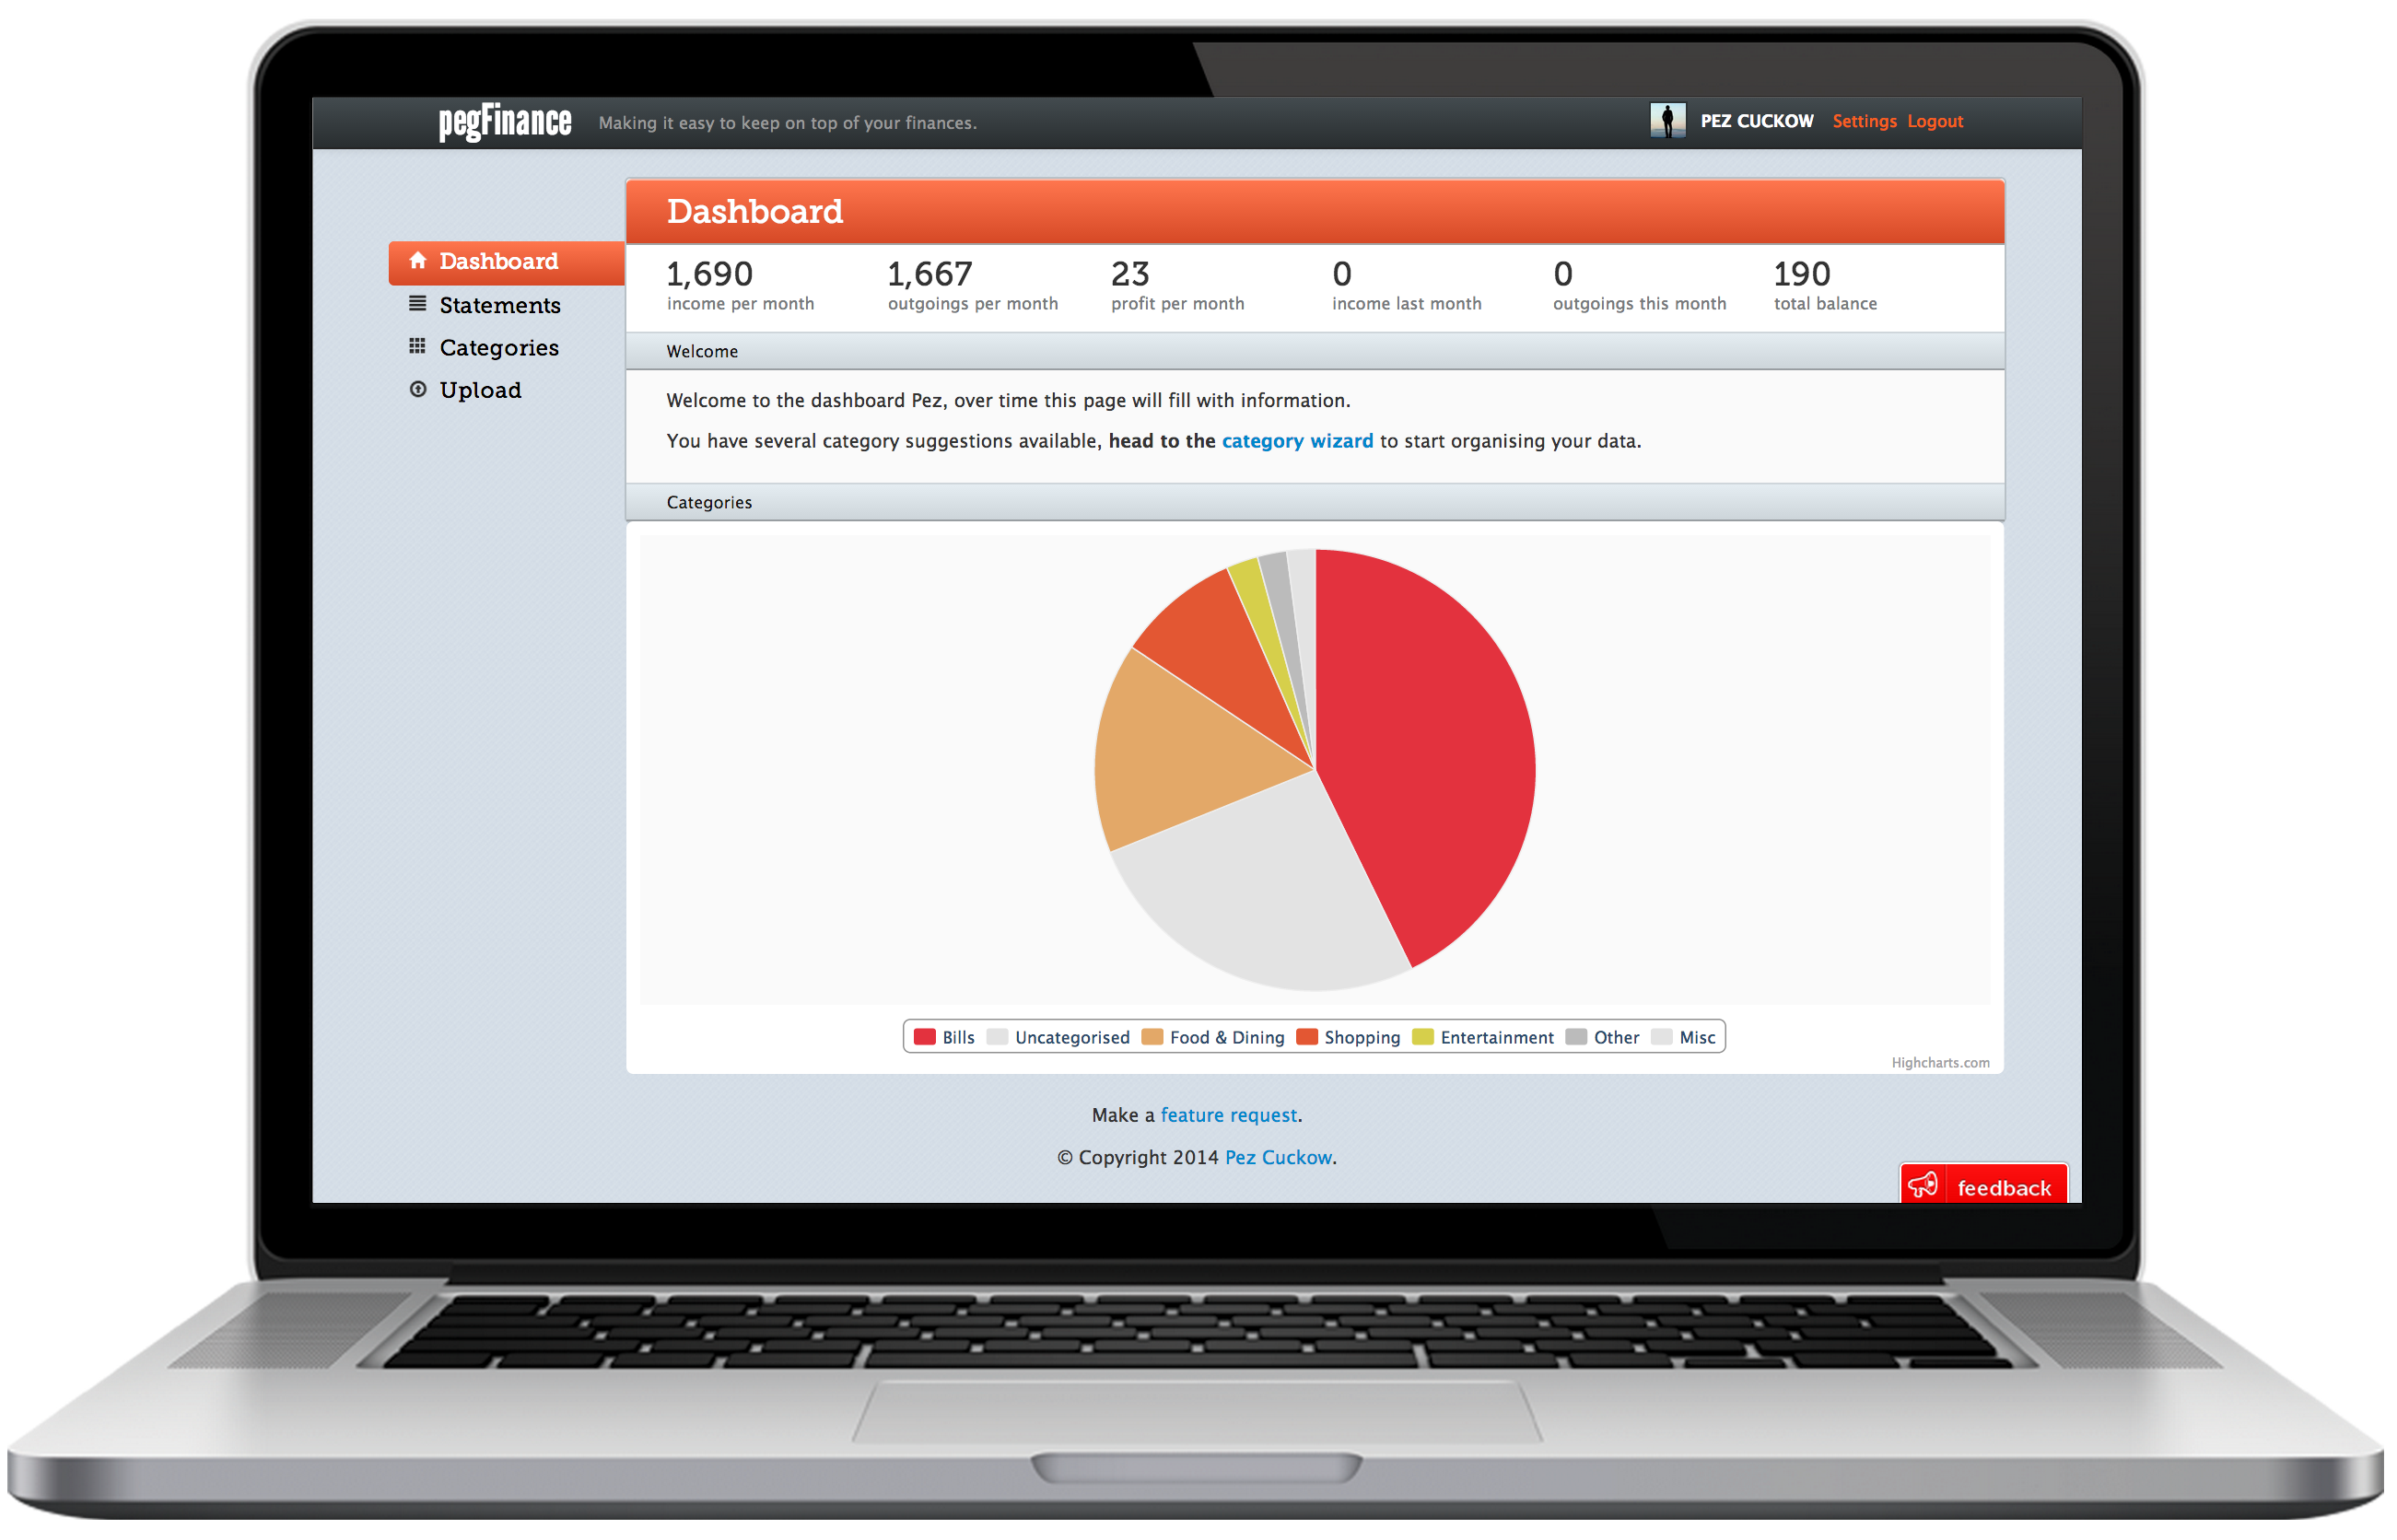
\includegraphics[width=0.8\textwidth]{screenshots/responsive/macbook}
    \caption{Layout on a standard laptop}
    \label{fig:responsive-macbook}
\end{figure}

\begin{figure}[h]
    \centering
    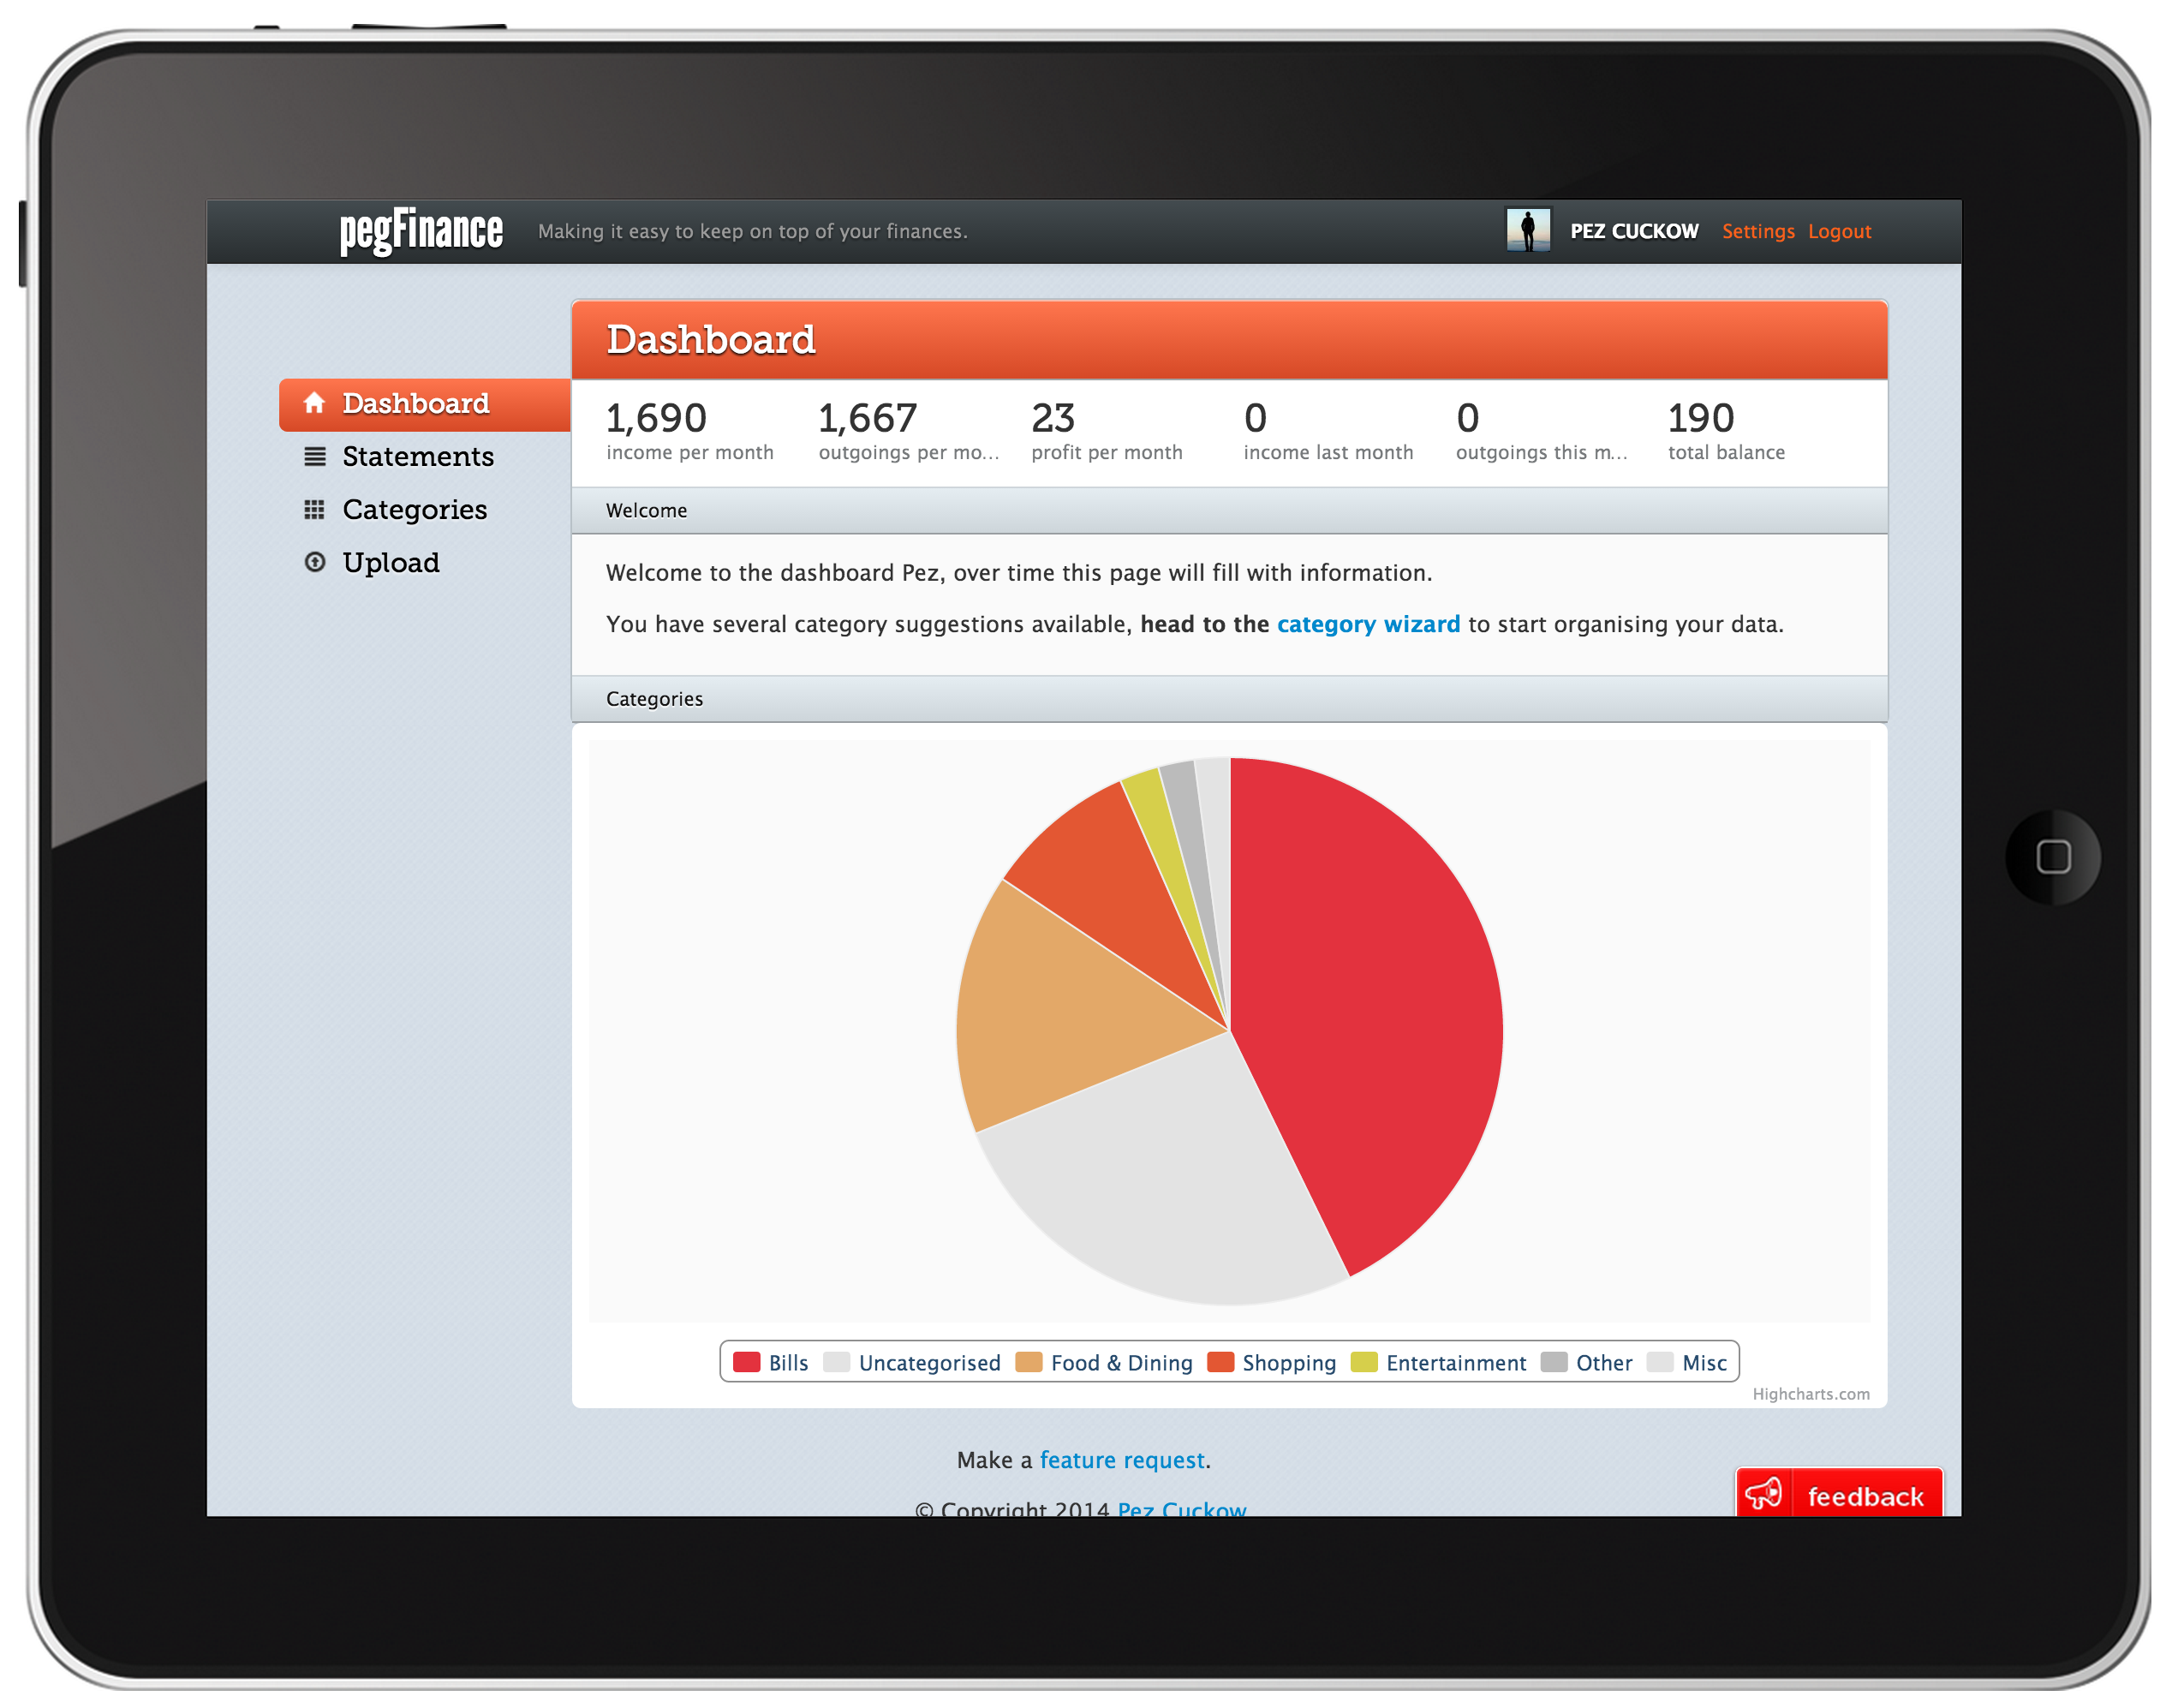
\includegraphics[width=0.8\textwidth]{screenshots/responsive/ipad-sideways}
    \caption{Layout on a tablet in landscape}
    \label{fig:responsive-ipad}
\end{figure}

\begin{figure}[h]
    \centering
    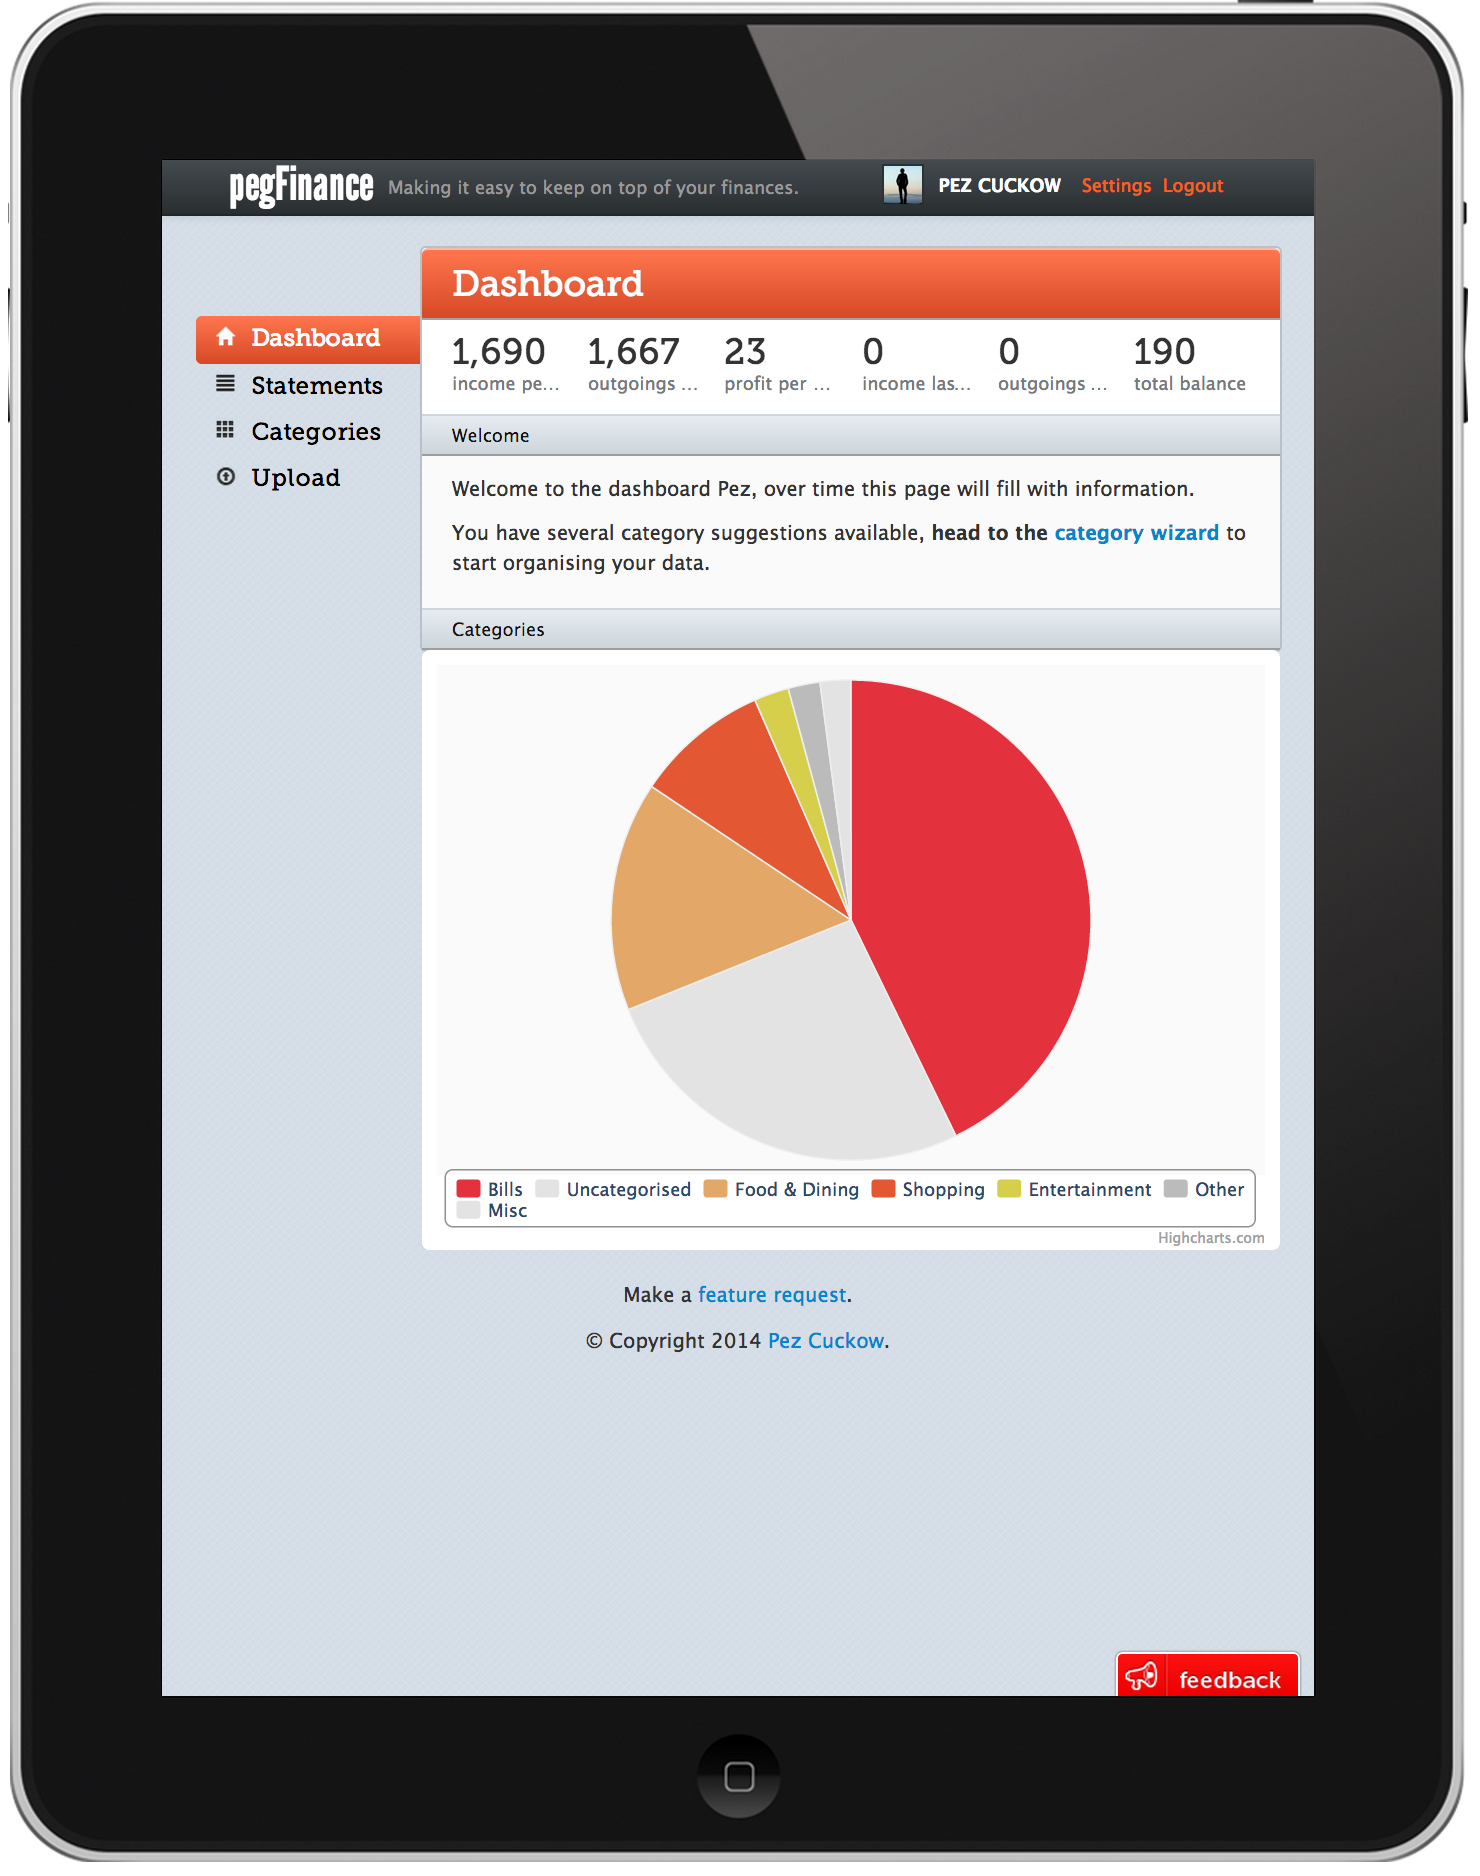
\includegraphics[width=0.5\textwidth]{screenshots/responsive/ipad-portrait}
    \caption{Layout on a tablet in portrait}
    \label{fig:responsive-ipad2}
\end{figure}

\begin{figure}[h]
    \centering
    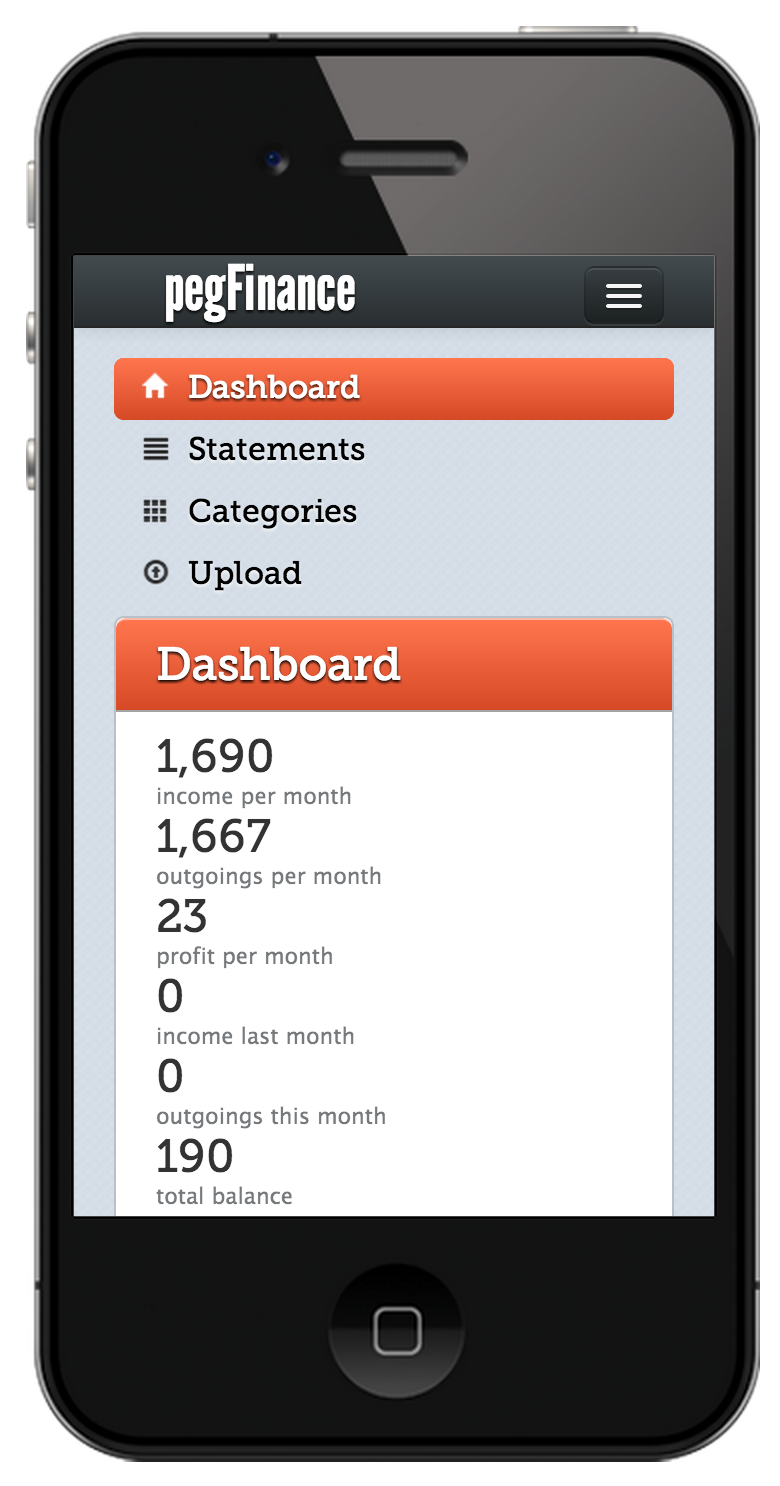
\includegraphics[width=0.5\textwidth]{screenshots/responsive/iphone-portrait}
    \caption{Layout on a smaller smartphone}
    \label{fig:responsive-iphone}
\end{figure}

%\section{Uploading a Statement}

%\section{Suggestion Engine}

%\section{Viewing Statements}

%\section{Prediction Overview}